% Retoca las líneas marcadas con TODO según las necesidades

\documentclass[oneside,a4paper,12pt]{book} % TODO: cambia "oneside" por "twoside" a la hora de imprimirlo

\usepackage[spanish]{babel}
\usepackage[utf8]{inputenc}
\usepackage{geometry}
\usepackage{makeidx}
\usepackage{url}
\usepackage{graphicx}
\usepackage{color}
\usepackage{caption}
\usepackage{acronym}
\usepackage{hyphenat}
\usepackage{a4wide}
\usepackage[normalsize]{subfigure}
\usepackage{float}
\usepackage{titlesec}
\usepackage[Lenny]{fncychap}
\usepackage{listings} % para poder hacer uso de "listings" propios (p.ej. códigos)
\usepackage{eurosym} % para poder usar el símbolo del euro con \euro {xx}
\usepackage{hyperref} % TODO: añade la opción hidelinks para imprimirlo (los enlaces no aparecerán resaltados)

% Para que no parta las palabras
\pretolerance=10000

\newcommand{\bigrule}{\titlerule[0.5mm]} \titleformat{\chapter}[display] % cambiamos el formato de los capítulos
{\bfseries\Huge} % por defecto se usaron caracteres de tamaño huge en negrita
{% contenido de la etiqueta 
\titlerule % línea horizontal 
\filright % texto alineado a la derecha 
\Large\chaptertitlename\ % capítulo e índice en tamaño large
\Large % en lugar de 
\Huge \Large\thechapter} 
{0mm} % espacio mínimo entre etiqueta y cuerpo
{\filright} % texto del cuerpo alineado a la derecha
[\vspace{0.5mm} \bigrule] % después del cuerpo, dejar espacio vertical y trazar línea horizontal gruesa
\geometry{a4paper, left=2.5cm, right=2.5cm, top=0.5cm, bottom=2.5cm, headsep=0.2cm}

% Estilos para ilustrar códigos:
\definecolor{code_green}{rgb}{0,0.6,0}
\definecolor{code_gray}{rgb}{0.5,0.5,0.5}
\definecolor{code_mauve}{rgb}{0.58,0,0.82}

\lstset{frame=tb,
  language=C,
  aboveskip=3mm,
  belowskip=3mm,
  showstringspaces=false,
  columns=flexible,
  basicstyle={\small\ttfamily},
  numbers=none,
  numberstyle=\tiny\color{code_gray},
  keywordstyle=\color{blue},
  commentstyle=\color{code_green},
  stringstyle=\color{code_mauve},
  breaklines=true,
  breakatwhitespace=true,
  tabsize=3
}

\lstset{frame=tb,
  language=C++,
  aboveskip=3mm,
  belowskip=3mm,
  showstringspaces=false,
  columns=flexible,
  basicstyle={\small\ttfamily},
  numbers=none,
  numberstyle=\tiny\color{code_gray},
  keywordstyle=\color{blue},
  commentstyle=\color{code_green},
  stringstyle=\color{code_mauve},
  breaklines=true,
  breakatwhitespace=true,
  tabsize=3
}

\lstset{frame=tb,
  language=Python,
  aboveskip=3mm,
  belowskip=3mm,
  showstringspaces=false,
  columns=flexible,
  basicstyle={\small\ttfamily},
  numbers=none,
  numberstyle=\tiny\color{code_gray},
  keywordstyle=\color{blue},
  commentstyle=\color{code_green},
  stringstyle=\color{code_mauve},
  breaklines=true,
  breakatwhitespace=true,
  tabsize=3
}

% Definición de mis propios tipos: Códigos, Ecuaciones y Tablas
\DeclareCaptionType{code}[Código][Listado de códigos]
\DeclareCaptionType{myequation}[Ecuación][Listado de ecuaciones]

% TODO: especifica las reglas de separación que consideres. Algunos ejemplos:
\hyphenation{fuer-tes}
\hyphenation{mul-ti-ca-pa}
\hyphenation{res-pues-ta}
\hyphenation{di-fe-ren-tes}
\hyphenation{de-sa-rro-lla-dos}
\hyphenation{re-pre-sen-tan-do}

 % archivo de configuración de estilo

\makeindex

\begin{document}
\baselineskip 1.35\baselineskip

\frontmatter

\thispagestyle{empty}
\vspace{2cm}

\begin{figure}[htb]
  \centerline{\resizebox{.60\textwidth}{!}{
\includegraphics{figs/logo_urjc}}}
\end{figure}

\begin{center}
  {\Large {\bf GRADO EN INGENIERÍA INFORMÁTICA}}
  \vspace{5mm}
 
  {\large {Escuela Técnica Superior de Ingeniería Informática}}
  \vspace{5mm}

  {\large {Curso académico 2022-2023}}

  \vspace{1cm}

  {\large {\bf Trabajo de Fin de Grado}}

  \vspace{2cm}

  {\Large {HERRAMIENTA SOFTWARE PARA \\
  LA UTILIZACIÓN DE NAVEGADORES INERCIALES\\[1cm] }}

  \vspace{5cm}
  {\bf Tutor}: Gustavo Recio Isasi \\
  {\bf Autor}: Juan Guillo Bermejo
\end{center}

\clearpage
\thispagestyle{empty}


% Este diseño se corresponde con la licencia CC-BY-NC-SA.
% Por supuesto, puedes poner la licencia que mejor se adapte al propósito de tu trabajo.
% Recuerda que, si no se especifica ninguna licencia, esta -como cualquier creación artística- pasaría a estar licenciada con todos los derechos reservados (copyright).

\cleardoublepage

\begin{figure}
 \ \ \ \ 
\includegraphics[width=0.25\linewidth]{figs/by-nc-sa.png}
 \label{fig:cc} 
 \end{figure}

\

\

\

\noindent
Este trabajo se distribuye bajo los términos de la licencia internacional \href{http://creativecommons.org/licenses/by-nc-sa/4.0/}{CC BY-NC-SA International License} (Creative Commons AttributionNonCommercial-ShareAlike 4.0). Usted es libre de \textit{(a) compartir}: copiar y redistribuir el material en cualquier medio o formato; y \textit{(b) adaptar}: remezclar, transformar y crear a partir del material. El licenciador no puede revocar estas libertades mientras cumpla con los términos de la licencia:

\begin{itemize}
\item \textit{Atribución}. Usted debe dar crédito de manera adecuada, brindar un enlace a la licencia, e indicar si se han realizado cambios. Puede hacerlo en cualquier forma razonable, pero no de forma tal que sugiera que usted o su uso tienen el apoyo de la licenciante.
\item \textit{No comercial}. Usted no puede hacer uso del material con propósitos comerciales.
\item \textit{Compartir igual}. Si remezcla, transforma o crea a partir del material, debe distribuir su contribución bajo la la misma licencia del original.
\end{itemize}

\begin{flushright}
		\vspace{7.0 cm}
		\emph{Documento de} \textbf{Juan Guillo Bermejo}. % TODO: pon aquí tu nombre cuando hagas el documento
\end{flushright}



\cleardoublepage

\chapter*{Agradecimientos}

Nunca se me había dado la ocasión de transmitir todo aquello que me ha permitido llegar hasta aquí, pero ha llegado la ocasión.\\

Desde luego que este primer comentario va hacia las personas que siempre han estado y sé que estarán como son mi familia. En especial a mis padres por darme todo lo que tengo, y como no, de mi hermano Pablo, el pequeño de la familia. Los pilares de mi vida.\\

Por aguantar la montaña rusa de emociones que causa y he ocasianado a lo largo de la carrera. Por otro lado, mencionar a mis amigos de toda la vida (Chipis), mis amigos del equipo de fútbol (Descanso FC), los cuales hemos vivido momentos inolvidables.\\

Mencionar a varios compañeros de la carrera por haberme acompañado durante éstos años.\\

Por último, agradecer a mi tutor Gustavo por darme la oportunidad y confiar en mí.\\

Gracias.\\
\ % Algo de separación...


\begin{flushright}
		\vspace{4.0 cm}
		\emph{A mi familia\\
      y amigos}\\
		\par
		\vspace{1.0 cm}
		Madrid, 15 de junio de 2023\\ %\today
		\emph{Juan}
\end{flushright}

\thispagestyle{empty}



\cleardoublepage

\chapter*{Resumen\markboth{Resumen}{Resumen}}

Escribe aquí el resumen del trabajo. Un primer párrafo para dar contexto sobre la temática que rodea al trabajo.\\

Un segundo párrafo concretando el contexto del problema abordado.\\

En el tercer párrafo, comenta cómo has resuelto la problemática descrita en el anterior párrafo.\\

Por último, en este cuarto párrafo, describe cómo han ido los experimentos.


\cleardoublepage

\chapter*{Acrónimos y palabras claves\markboth{Acrónimos y palabras claves}{Acrónimos y palabras claves}}

% Añade a continuación los acrónimos que uses en el documento. Algunos ejemplos:
\begin{acronym}
\acro{URJC}{\emph{Universidad Rey Juan Carlos}}
\acro{IMU}{\emph{Unidad de Medición Inercial}}
\acro{AHRS}{\emph{Attitude and Heading Reference Systems}}
\acro{LiDAR}{\emph{Light Detection and Ranging o Laser Imaging Detection and Ranging}}
\acro{Adafruit BNO055}{\emph{Ejemplo}}
\acro{Arduino}{\emph{Ejemplo}}
\acro{Infrared Laser Sensor}{\emph{Ejemplo}}
\acro{IDII}{\emph{Ivrea Interaction Design Institute}}
\acro{Parte Hardware}{\emph{Ejemplo}}
\acro{Parte Software}{\emph{Ejemplo}}
\end{acronym}


\cleardoublepage

\tableofcontents

\listoffigures

\listofcodes

\listofmyequations

\listoftables

%\pagestyle{empty}

\cleardoublepage

 % aquí se cargan todas las "primeras páginas"

% Bibliografía
\let\OLDthebibliography=\thebibliography
\def\thebibliography#1{\OLDthebibliography{#1}
  \addcontentsline{toc}{chapter}{\bibname}}

\mainmatter

\setcounter{page}{1}
\chapter{Introducción}
\label{cap:capitulo1}
\setcounter{page}{1}

Escribe aquí un párrafo explicando brevemente lo que vas a contar en este capítulo. En este primer capítulo, el de introducción, se trata de dar un contexto amplio y atractivo del trabajo. Comienza hablando de un contexto general y acaba hablando del contexto más específico en el que se enmarca el proyecto. Es el capítulo idóneo para incluir todas las referencias bibliográficas que hayan tratado este tema; suponen un fuerte respaldo al trabajo.\\

\section{La primera sección}
\label{sec:miseccion} % etiqueta para luego referenciar esta sección

En los textos puedes poner palabras en \textit{cursiva}, para aquellas expresiones en sentido \textit{figurado}, palabras como \textit{robota}, que está fuera del diccionario castellano, o bien para resaltar palabras de una colección: \textit{(a)} es la primera letra del abecedario, \textit{(b)} es la segunda, etc.\\

Al poner las dos líneas del anterior párrafo, este aparecerá separado del anterior. Si no las pongo, los párrafos aparecerán pegados. Sigue el criterio que consideres más oportuno.

\section{Segunda sección}
\label{sec:segundaseccion}

No olvides incluir imágenes y referenciarlas, como la Figura \ref{fig:mpu-9250}.

\begin{figure} [h!]
  \begin{center}
    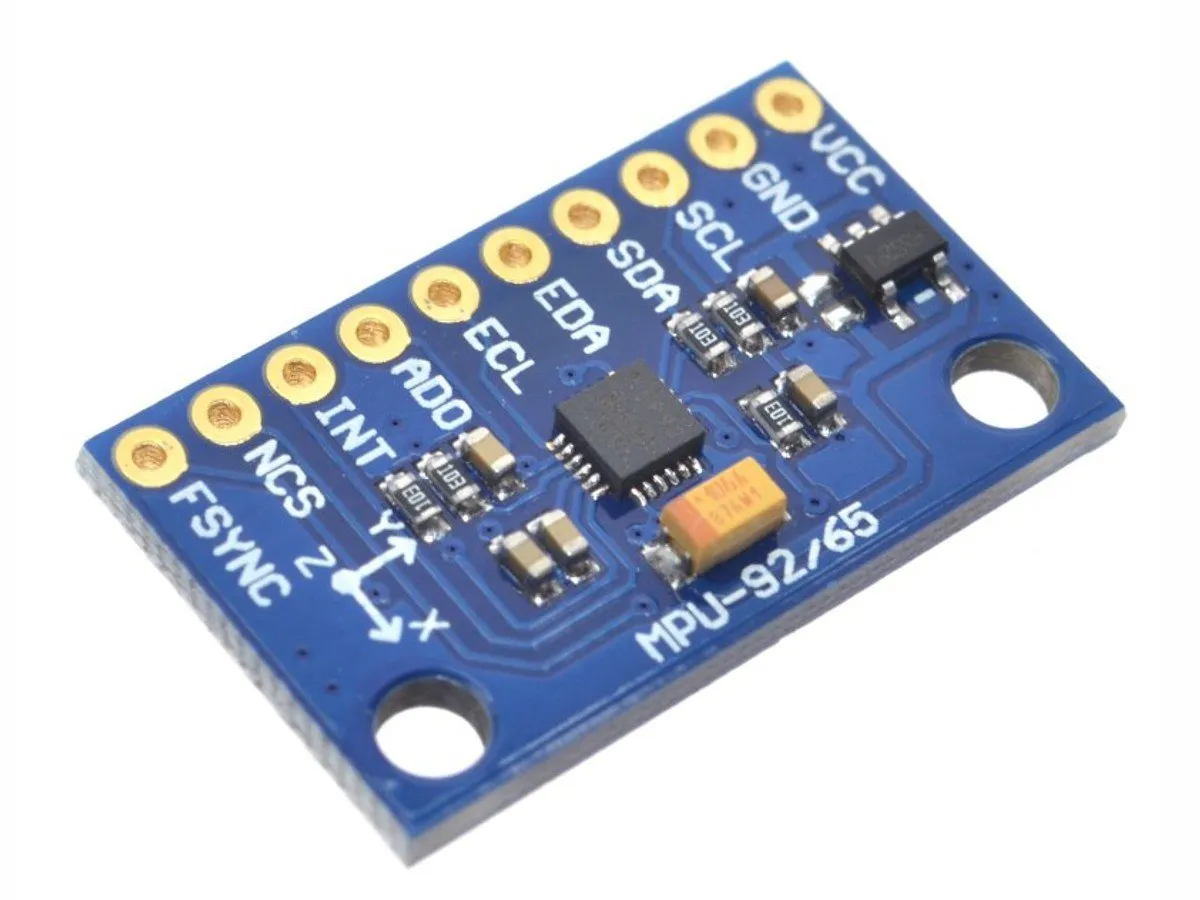
\includegraphics[width=8cm]{figs/mpu-9250}
  \end{center}
  \caption{Disposito MPU-9250.}
  \label{fig:mpu-9250}
\end{figure}\

Ni tampoco olvides de poner las URLs como notas al pie. Por ejemplo, si hablo de la Robocup\footnote{\url{http://www.robocup.org}}.

\subsection{Números}
\label{sec:subseccion}

En lugar de tener secciones interminables, como la Sección \ref{sec:miseccion}, divídelas en subsecciones.

Para hablar de números, mételos en el entorno \textit{math} de \LaTeX, por ejemplo, $1.5Kg$. También puedes usar el símbolo del Euro como aquí: 1.500\euro.

\subsection{Listas}

Cuando describas una colección, usa \texttt{itemize} para ítems o \texttt{enumerate} para enumerados. Por ejemplo:

\begin{itemize}
 \item \textit{Entorno de simulación.} Hemos usado dos entornos de simulación: uno en 3D y otro en 2D.
 \item \textit{Entornos reales.} Dentro del campus, hemos realizado experimentos en Biblioteca y en el edificio de Gestión.
\end{itemize}\

\begin{enumerate}
 \item Primer elemento de la colección.
 \item Segundo elemento de la colección.
\end{enumerate}\

\paragraph{Referencias bibliográficas}
\label{sec:referencias}

Cita, sobre todo en este capítulo, referencias bibliográficas que respalden tu argumento. Para citarlas basta con poner la instrucción \verb|\cite| con el identificador de la cita. Por ejemplo: libros como \cite{vega12e}, artículos como \cite{vega19b}, URLs como \cite{vega19a}, tesis como \cite{vega18b}, congresos como \cite{vega18a}, u otros trabajos fin de grado como \cite{vega08b}.

Las referencias, con todo su contenido, están recogidas en el fichero \texttt{bibliografia.bib}. El contenido de estas referencias está en formato \texttt{BibTex}. Este formato se puede obtener en muchas ocasiones directamente, desde plataformas como \texttt{Google Scholar} u otros repositorios de recursos científicos.

Existen numerosos estilos para reflejar una referencia bibliográfica. El estilo establecido por defecto en este documento es APA, que es uno de los estilos más comunes, pero lo puedes modificar en el archivo \texttt{memoria.tex}; concretamente, cambiando el campo \verb|apalike| a otro en la instrucción \verb|\bibliographystyle{apalike}|. 




\

\

\

Y, para terminar este capítulo, resume brevemente qué vas a contar en los siguientes.


\chapter{Objetivos}
\label{cap:capitulo2}


Escribe aquí un párrafo explicando brevemente lo que vas a contar en este capítulo. En este capítulo lo ideal es explicar cuáles han sido los objetivos que te has fijado conseguir con tu trabajo, qué requisitos ha de respetar el resultado final, y cómo lo has llevado a cabo; esto es, cuál ha sido tu plan de trabajo.\\

\section{Descripción del problema}
\label{sec:descripcion}

Cuenta aquí el objetivo u objetivos generales y, a continuación, concrétalos mediante objetivos específicos.

\section{Requisitos}
\label{sec:requisitos}

Describe los requisitos que ha de cumplir tu trabajo.

\section{Metodología}
\label{sec:metodologia}

Qué paradigma de desarrollo software has seguido para alcanzar tus objetivos.

\section{Plan de trabajo}
\label{sec:plantrabajo}

Qué agenda has seguido. Si has ido manteniendo reuniones semanales, cumplimentando objetivos parciales, si has ido afinando poco a poco un producto final completo, etc.


\chapter{Descripción informática}
\label{cap:capitulo3}


Escribe aquí un párrafo explicando brevemente lo que vas a contar en este capítulo. En este capítulo (y quizás alguno más) es donde, por fin, describes detalladamente qué has hecho y qué experimentos has llevado a cabo para validar tus desarrollos (con el siguiente capítulo explico detalladamente esto).

\section{Especificación}

Puede resultar interesante, para clarificar la descripción, mostrar fragmentos de código (o \textit{snippets}) ilustrativos. En el Código \ref{cod:codejemplo} vemos un ejemplo escrito en \texttt{C++}.

\section{Diseño}

\section{Implementación}

Si necesitas insertar alguna ecuación, puedes hacerlo. Al igual que las figuras, no te olvides de referenciarlas. A continuación se exponen algunas ecuaciones de ejemplo: Ecuación \ref{ec:ec1} y Ecuación \ref{ec:ec2}.

\section{Pruebas}




\chapter{Descripción informática}
\label{cap:capitulo4}


Escribe aquí un párrafo explicando brevemente lo que vas a contar en este capítulo. En este capítulo (y quizás alguno más) es donde, por fin, describes detalladamente qué has hecho y qué experimentos has llevado a cabo para validar tus desarrollos.

\section{Especificación}

Puede resultar interesante, para clarificar la descripción, mostrar fragmentos de código (o \textit{snippets}) ilustrativos. En el Código \ref{cod:codejemplo} vemos un ejemplo escrito en \texttt{C++}.

\begin{code}[h]
\begin{lstlisting}[language=C++]
void Memory::hypothesizeParallelograms () {
  for(it1 = this->controller->segmentMemory.begin(); it1++) {
    squareFound = false; it2 = it1; it2++;
    while ((it2 != this->controller->segmentMemory.end()) && (!squareFound)) {
      if (geometry::haveACommonVertex((*it1),(*it2),&square)) {
        dist1 = geometry::distanceBetweenPoints3D ((*it1).start, (*it1).end);
        dist2 = geometry::distanceBetweenPoints3D ((*it2).start, (*it2).end);
      }
    // [...]
\end{lstlisting}
\caption[Función para buscar elementos 3D en la imagen]{Función para buscar elementos 3D en la imagen}
\label{cod:codejemplo}
\end{code}

En el Código \ref{cod:codejemplo2} vemos un ejemplo escrito en \texttt{Python}.

\begin{code}[h]
\begin{lstlisting}[language=Python]
def mostrarValores():
    print (w1.get(), w2.get())

master = Tk()
w1 = Scale(master, from_=0, to=42)
w1.pack()
w2 = Scale(master, from_=0, to=200, orient=HORIZONTAL)
w2.pack()
Button(master, text='Show', command=mostrarValores).pack()

mainloop()
\end{lstlisting}
\caption[Cómo usar un Slider]{Cómo usar un Slider}
\label{cod:codejemplo2}
\end{code}

\section{Diseño}

Para mencionar identificadores usados en el código ---como nombres de funciones o variables--- en el texto, usa el entorno literal o verbatim \verb|hypothesizeParallelograms()|. También se puede usar este entorno para varias líneas, como se ve a continuación:

\begin{verbatim}
void Memory::hypothesizeParallelograms () {
  // add your code here
}
\end{verbatim}

\section{Implementación}

Si necesitas insertar alguna ecuación, puedes hacerlo. Al igual que las figuras, no te olvides de referenciarlas. A continuación se exponen algunas ecuaciones de ejemplo: Ecuación \ref{ec:ec1} y Ecuación \ref{ec:ec2}.

\begin{myequation}[h]
\begin{equation}
H = 1 - \frac{\sum_{i=0}^{N}\frac{(\frac{d_{j_s} + d_{j_e}}{2})}{N}}{M}
\nonumber
\label{ec:ec1}
\end{equation}
\caption[Ejemplo de ecuación con fracciones]{Ejemplo de ecuación con fracciones}
\end{myequation} 

\begin{myequation}[h]
\begin{equation}
v(entrada)= \left\{
	\begin{array}{lcc}
		0 & \mbox{if} & \epsilon_t < 0.1\\
		K_p\cdot{(T_{t}-T)} & \mbox{if}& 0.1 \leq \epsilon_t < M_t\\
		K_p \cdot M_t & \mbox{if}& M_t < \epsilon_t
	\end{array}
\right.
\label{ec:ec2}
\end{equation}
\caption[Ejemplo de ecuación con array y letras y símbolos especiales]{Ejemplo de ecuación con array y letras y símbolos especiales}
\end{myequation}

\section{Pruebas}

Si necesitas insertar una tabla, hazlo dígnamente usando las propias tablas de \LaTeX, no usando pantallazos e insertándolas como figuras... En el Cuadro \ref{cuadro:ejemplo} vemos un ejemplo.

\begin{table}[H]
\begin{center}
\begin{tabular}{|c|c|}
\hline
\textbf{Parámetros} & \textbf{Valores} \\
\hline
Tipo de sensor & Sony IMX219PQ[7] CMOS 8-Mpx \\
Tamaño del sensor & 3.674 x 2.760 mm (1/4" format) \\
Número de pixels & 3280 x 2464 (active pixels) \\
Tamaño de pixel & 1.12 x 1.12 um \\
Lente & f=3.04 mm, f/2.0 \\
Ángulo de visión & 62.2 x 48.8 degrees \\
Lente SLR equivalente & 29 mm \\
\hline
\end{tabular}
\caption{Parámetros intrínsecos de la cámara}
\label{cuadro:ejemplo}
\end{center}
\end{table}



\chapter{Conclusiones}
\label{cap:capitulo5}

\begin{flushright}
\begin{minipage}[]{10cm}
\emph{Quizás algún fragmento de libro inspirador...}\\
\end{minipage}\\

Autor, \textit{Título}\\
\end{flushright}

\vspace{1cm}

Escribe aquí un párrafo explicando brevemente lo que vas a contar en este capítulo, que básicamente será una recapitulación de los problemas que has abordado, las soluciones que has prouesto, así como los experimentos llevados a cabo para validarlos. Y con esto, cierras la memoria.

\section{Conclusiones}

Enumera los objetivos y cómo los has cumplido.\\

Enumera también los requisitos implícitos en la consecución de esos objetivos, y cómo se han satisfecho.\\

No olvides dedicar un par de párrafos para hacer un balance global de qué has conseguido, y por qué es un avance respecto a lo que tenías inicialmente. Haz mención expresa de alguna limitación o peculiaridad de tu sistema y por qué es así. Y también, qué has aprendido desarrollando este trabajo.\\

Por último, añade otro par de párrafos de líneas futuras; esto es, cómo se puede continuar tu trabajo para abarcar una solución más amplia, o qué otras ramas de la investigación podrían seguirse partiendo de este trabajo, o cómo se podría mejorar para conseguir una aplicación real de este desarrollo (si es que no se ha llegado a conseguir).

\section{Corrector ortográfico}

Una vez tengas todo, no olvides pasar el corrector ortográfico de \LaTeX a todos tus ficheros \textit{.tex}. En \texttt{Windows}, el propio editor \texttt{TeXworks} incluye el corrector. En \texttt{Linux}, usa \texttt{aspell} ejecutando el siguiente comando en tu terminal:

\begin{verbatim}
aspell --lang=es --mode=tex check capitulo1.tex
\end{verbatim}


\chapter{Conclusiones}
\label{cap:capitulo6}

\begin{flushright}
\begin{minipage}[]{10cm}
\emph{Quizás algún fragmento de libro inspirador...}\\
\end{minipage}\\

Autor, \textit{Título}\\
\end{flushright}

\vspace{1cm}

Escribe aquí un párrafo explicando brevemente lo que vas a contar en este capítulo, que básicamente será una recapitulación de los problemas que has abordado, las soluciones que has prouesto, así como los experimentos llevados a cabo para validarlos. Y con esto, cierras la memoria.

\section{Posibles mejoras}

Enumera los objetivos y cómo los has cumplido.\\

Enumera también los requisitos implícitos en la consecución de esos objetivos, y cómo se han satisfecho.\\

No olvides dedicar un par de párrafos para hacer un balance global de qué has conseguido, y por qué es un avance respecto a lo que tenías inicialmente. Haz mención expresa de alguna limitación o peculiaridad de tu sistema y por qué es así. Y también, qué has aprendido desarrollando este trabajo.\\

Por último, añade otro par de párrafos de líneas futuras; esto es, cómo se puede continuar tu trabajo para abarcar una solución más amplia, o qué otras ramas de la investigación podrían seguirse partiendo de este trabajo, o cómo se podría mejorar para conseguir una aplicación real de este desarrollo (si es que no se ha llegado a conseguir).



\chapter{Anexos}
\label{cap:capitulo7}

\begin{flushright}
\begin{minipage}[]{10cm}
\emph{Quizás algún fragmento de libro inspirador...}\\
\end{minipage}\\

Autor, \textit{Título}\\
\end{flushright}

\vspace{1cm}

Escribe aquí un párrafo explicando brevemente lo que vas a contar en este capítulo, que básicamente será una recapitulación de los problemas que has abordado, las soluciones que has prouesto, así como los experimentos llevados a cabo para validarlos. Y con esto, cierras la memoria.

\section{Información de interés}

Enumera los objetivos y cómo los has cumplido.\\

Enumera también los requisitos implícitos en la consecución de esos objetivos, y cómo se han satisfecho.\\

No olvides dedicar un par de párrafos para hacer un balance global de qué has conseguido, y por qué es un avance respecto a lo que tenías inicialmente. Haz mención expresa de alguna limitación o peculiaridad de tu sistema y por qué es así. Y también, qué has aprendido desarrollando este trabajo.\\

Por último, añade otro par de párrafos de líneas futuras; esto es, cómo se puede continuar tu trabajo para abarcar una solución más amplia, o qué otras ramas de la investigación podrían seguirse partiendo de este trabajo, o cómo se podría mejorar para conseguir una aplicación real de este desarrollo (si es que no se ha llegado a conseguir).

%\section{Corrector ortográfico}

%Una vez tengas todo, no olvides pasar el corrector ortográfico de \LaTeX a todos tus ficheros \textit{.tex}. En \texttt{Windows}, el propio editor \texttt{TeXworks} incluye el corrector. En \texttt{Linux}, usa \texttt{aspell} ejecutando el siguiente comando en tu terminal:

%\begin{verbatim}
%aspell --lang=es --mode=tex check capitulo1.tex
%\end{verbatim}


\clearpage
\thispagestyle{empty}

\printindex \nocite{*}
\appendix
\bibliographystyle{apalike} \bibliography{bibliografia}

\end{document}
